\documentclass[usenames, aspectratio=169]{beamer}

\usepackage{amsmath}
\usepackage{braket}
\usepackage{amsfonts}
\usepackage{tikz}
\usepackage{tkz-graph}
\usepackage{tikzpeople}
\usepackage{adjustbox}
\usepackage{subcaption}
\usepackage{svg}
\usepackage{graphicx}
\usepackage{media9}
\usepackage{float}
\usetikzlibrary{calc}
\usepackage{array}
\usepackage{efbox,graphicx}
\usepackage[normalem]{ulem}
\usepackage{verbatim}
\usepackage{ragged2e}
\usepackage{array}
\usepackage[backend=biber,style=alphabetic,sorting=ynt]{biblatex}
\addbibresource{./sample.bib} 
  
\efboxsetup{linecolor=Green,linewidth=1.5pt, margin=0pt}

\usetikzlibrary{decorations.pathreplacing}

\newcommand\MemoryLayout[1]{
  \begin{tikzpicture}[scale=0.15]
    \draw[thick](0,0)--++(0,3)node[above]{$0$};
    \foreach \pt/\col/\lab [remember=\pt as \tp (initially 0)] in {#1} {
      \foreach \a [parse=true] in {\tp,...,\pt-1} {
        \draw[fill=\col](-\a, 0) rectangle ++(-1,2);
      }
      \draw[thick](-\pt,0)--++(0,3)node[above]{$\pt$};
      \if\lab\relax\relax\else
        \draw[thick,decorate, decoration={amplitude=1mm}]
        (-\tp,-0.2)--node[below=1mm]{\lab} (-\pt,-0.2);
      \fi
    }
  \end{tikzpicture}
}


\newcommand{\pslsq}[4]{
\begin{frame}
    \frametitle{#1} 
    \includegraphics[width=.7\linewidth]{#3}
    #4  
  \end{frame}
}

\newcommand{\psls}[4]{
  \begin{frame}
    \frametitle{#1} 
    \begin{columns}[t]
      \begin{column}{.48\textwidth}
        #4
      \end{column}
      \begin{column}{.52\textwidth}
        \adjincludegraphics[width=.98\linewidth, valign=t]{#3}
      \end{column} 
    \end{columns}
  \end{frame}
}
\newcommand{\commentt}[1]{\textcolor{blue}{ \textbf{[COMMENT]} #1}}
\newcommand{\ctt}[1]{\commentt{#1}}
\newcommand{\prb}[1]{ \mathbf{Pr} \left[ #1 \right]}
\newcommand{\prbm}[2]{ \mathbf{Pr}_{ #2 }\left[ #1 \right]}
\newcommand{\prbc}[3]{ \mathbf{Pr}_{ #2 }\left[ #1 \right | #3]}
\newcommand{\prbcprb}[3]{ \prbc{#2}{#1}{#3} \cdot \prb{#3} } 
\newcommand{\expp}[1]{ \mathbf{E} \left[ {#1} \right]}
\newcommand{\onotation}[1]{\(\mathcal{O} \left( {#1}  \right) \)}
\newcommand{\ona}[1]{\onotation{#1}}
\newcommand{\PSI}{{\ket{\psi}}}
\newcommand{\xij} { X_{ij} } 
\DeclareMathOperator{\Ima}{Im}
%\newcommand{\LESn}{\ket{\psi_n}}
%\newcommand{\LESa}{\ket{\phi_n}}
%\newcommand{\LESs}{\frac{1}{\sqrt{n}}\sum_{i}{\ket{\left(0^{i}10^{n-i}\right)^{n}}}}
%\newcommand{\Hn}{\mathcal{H}_{n}}
%\newcommand{\Ep}{\frac{1}{\sqrt{2^n}}\sum^{2^n}_{x}{ \ket{xx}}}
%\newcommand{\HON}{\ket{\psi_{\text{honest}}}}
%\newcommand{\Lemma}{\paragraph{Lemma.}}
\newcommand{\Cpa}{[n, \rho n, \delta n]}
%\setlength{\columnsep}{0.6cm}
\newcommand{\Jvv}{ \bar{J_{v}} } 
\newcommand{\Cvv}{ \tilde{C_{v}} } 

\newcommand{\Gz}{ G_{z}^{\delta} } 
\newcommand{ \Tann } {  \mathcal{T}\left( G, C_0 \right) }
\newcommand{\ireducable}{ireducable \hyperref[ire]{[\ref{ire}]} }
\newcommand{\cutUU}{E(U_{-1} \bigcup U_{+1} ,U)} 
\newcommand{\wcutUU}{w\left( E(U_{-1} \bigcup U_{+1} ,U)  \right)}
\newcommand{\testgo}{  \mathcal{T}\left(J, q , C_{0}\right) } 

\newcommand{\duC}{\left( C_{A}^{\perp}\otimes C_{B}^{\perp} \right)^{\perp}}
\newcommand{\duduC}{\left( C_{A}\otimes C_{B}\right)^{\perp}}
  




\usepackage{sagetex}
%\usepackage{libertine}
%\usepackage{emerald}
%\usepackage[T1]{fontenc}
\usetheme[progressbar=frametitle]{metropolis}
\setbeamercolor{block title}{use=structure,fg=white,bg=structure.fg!75!black}
\setbeamercolor{block body}{parent=normal text,use=block title,bg=block title.bg!10!bg}

%\usetheme{EastLansing}
\title[From classical to quantum good LDPC codes.] % (optional, only for long titles)
{From classical to quantum good LDPC codes.}

\subtitle{  }
\author[D.~Ponarovsky] % (optional, for multiple authors)
	{D.~Ponarovsky\inst{1}}

\institute[HUJI] % (optional)
{  Faculty of Computer Science\newline
  Hebrew University of Jerusalem
}
\date[2023] % (optional)
{Master-Exam-Huji.}
\subject{Understanding Quantumness And Testability.}

\begin{document}
\input{sageutil.py}

\tikzset{
    LabelStyle/.append style = {  minimum width = 2em},
    VertexStyle/.append style = { inner sep=5pt,
        font = \Large\bfseries},
    EdgeStyle/.append style = {->} % added blue
}

\begin{frame}
  \maketitle
\end{frame}
%\pslsq{Today.}{0.3}{controller.png}{}
%\pslsq{Today.}{0.5}{controller-2-out.png}{}

\begin{frame}
  \frametitle{ Today. }
  \begin{itemize}
    \item<1-> Brif Review of Coding. \uncover<2->{Tanner and Expander codes. }
    \item<3-> Quantum Error Correction Codes. 
    \item<4->Good Classical Locally Testabile Codes and Good Qauntum LDPC.
  \end{itemize} 
\end{frame}


\begin{frame}
  \begin{center}
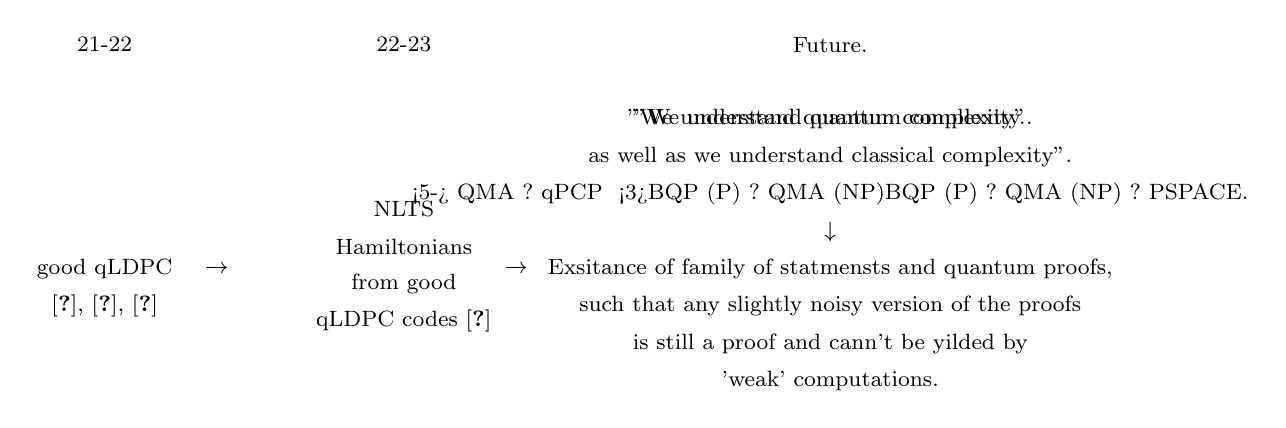
\begin{tikzpicture}[scale=0.95]

  \tikzset{
  font={\fontsize{8pt}{12}\selectfont}}

  \draw (13.7,6) node { Future. };
  \alt<4->{ 
    \draw (13.7,5) node { ''We understand quantum complexity. };
    \draw (13.7,4.5) node { as well as we understand classical complexity''. };
}{\draw (13.7,5) node { ''We understand quantum complexity''. };}
\uncover<3-> {\draw (13.7,4) node { \alt<5->{  QMA ? qPCP }{ \alt<3>{BQP (P) ? QMA (NP)}{BQP (P) ? QMA (NP)} ? PSPACE. }};}
\uncover<7->{\draw (13.7,3.5) node { $\downarrow$ };}
\uncover<8->{
  \draw (13.7,3) node { Exsitance of family of statmensts and quantum proofs, };
\draw (13.7,2.5) node {  such that any slightly noisy version of the proofs   };
\draw (13.7,2) node {  is still a proof and cann't be yilded by };
\draw (13.7,1.5) node { 'weak' computations. };
}
\uncover<8->{
  \draw (9.5,3) node { $\rightarrow$ };
  \draw (8,3.8) node { NLTS };
  \draw (8,3.3) node { Hamiltonians };
  \draw (8,2.8) node { from good};
  \draw (8,2.3) node { qLDPC codes \cite{anshu2022nlts}};
  \draw (8,6) node { 22-23 };
}
\uncover<9->{
  \draw (5.5,3) node { $\rightarrow$ };
  \draw (4,3) node { good qLDPC };
  \draw (4,2.5) node { \cite{Dinur}, \cite{Pavel}, \cite{leverrier2022quantum} };
  \draw (4,6) node { 21-22 };
}

        \end{tikzpicture}
    \end{center}
\end{frame}



\begin{frame}
  \frametitle{Introduction.}
  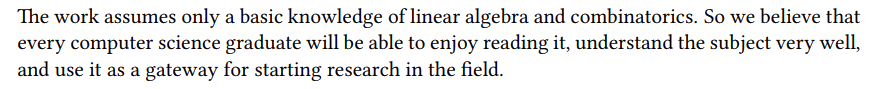
\includegraphics[width=.7\linewidth]{./Assumption-out.png}
\end{frame}



\begin{frame}
  \frametitle{ Coding. }
  \begin{center}
  \begin{tikzpicture}
    \node[name=b, bob,monitor,minimum size=1cm,xshift=-7.2cm]{};
    \node[name= a, alice,monitor, mirrored,minimum size=1cm]{};
    \node (C) at (-2,0) {};
    \node (E) at ( (a.mouth.x) -1, (a.mouth.y) ) {}; 
    \draw[ -> ] (b.mouth) + (1,0) to (a.mouth); 
    \alt<2->{ \node (D) at (-4,1) { $1\textcolor{red}{0}0101$ } ; }{\node (D) at (-4,1) { $110101$ } ; } 
    \uncover<3->{ \node (D) at (-3.4,1.5) { $1\textcolor{red}{0}0101 1\textcolor{red}{1}0101$ } ; }  
    %\uncover<2->{\node (D) at (-4,1) { $110101$ } ;  
  \end{tikzpicture}
\end{center}
\end{frame}

\begin{frame}
  \frametitle{ Coding. }
  Can we come up with a code that tolerates $*$ bits flip? 
\end{frame} 

\begin{frame}
  \frametitle{ Coding. }
\begin{definition} 
  Let $n \in \mathbb{N}$ and $\rho, \delta\in \left( 0,1 \right)$. We say that $C$ is a \textbf{binary linear code} with parameters $[n, \rho n, \delta n]$. If $C$ is a subspace of $\mathbb{F}_{2}^{n}$, and the dimension of $C$ is at least $\rho n$. In addition, we call the vectors belong to $C$ \textit{codewords} and define the distance of $C$ to be the minimal number of different bits between any codewords pair of $C$.   
  \end{definition}
\end{frame} 

\begin{frame}
  \frametitle{ Coding. }
\begin{definition} 
  A \textbf{family of codes} is an infinite series of codes. Additionally, suppose the rates and relative distances converge into constant values $\rho,\delta$. In that case, we abuse the notation and call that family of codes a code with $[n, \rho n, \delta n]$ for fixed $\rho, \delta\in [ 0,1 )$, and infinite integers $n \in \mathbb{N}$.     
  \end{definition}
\begin{definition} 
  We will say that a family of codes is a \textbf{good code} if its parameters converge into positive values. 
  \end{definition}
\end{frame} 

\begin{frame}
  \frametitle{ Tanner Codes. }
  \begin{definition} Let $\Gamma$ be a graph and $C_{0}$ be a ``small'' linear code with finate parameters $[\Delta, \rho\Delta, \delta\Delta]$. Let $ C = \mathcal{T}\left( \Gamma, C_{0} \right)$  be all the codewords which, for any vertex $v\in \Gamma$, the local view of $v$ is a codeword of $C_{0}$. We say that $C$ is a \textbf{Tanner code}\label{Tan} of $\Gamma, C_{0}$. Notice that if $C_{0}$ is a binary linear code, So $C$ is.  
  \end{definition}
\end{frame}


\begin{frame}
  \frametitle{ Tanner Codes. }
  Example, the parity code on the Peterson graph.
  \begin{center}
  \scalebox{0.65} {
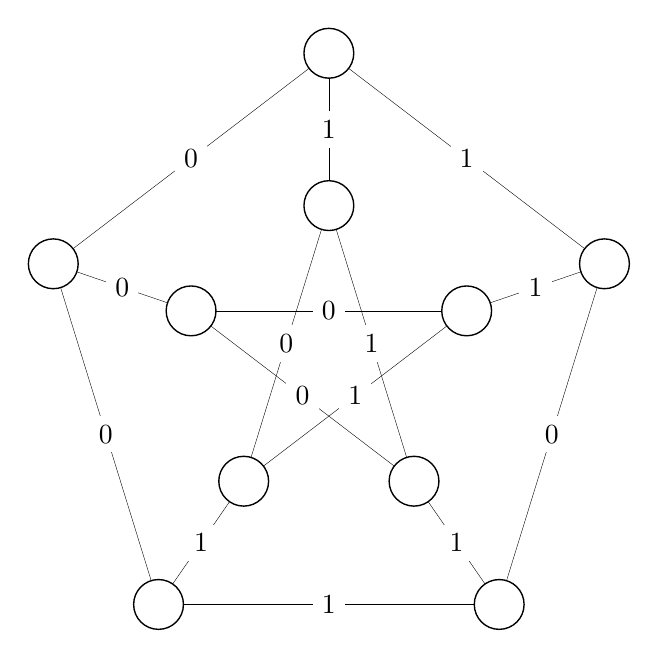
\begin{tikzpicture}

\Vertex[style={minimum size=0.01cm,shape=circle},NoLabel,x=3.5cm,y=7.0cm]{v0}
\Vertex[style={minimum size=0.01cm,shape=circle},NoLabel,x=0.0cm,y=4.3262cm]{v1}
\Vertex[style={minimum size=0.01cm,shape=circle},NoLabel,x=1.3369cm,y=0.0cm]{v2}
\Vertex[style={minimum size=0.01cm,shape=circle},NoLabel,x=5.6631cm,y=0.0cm]{v3}
\Vertex[style={minimum size=0.01cm,shape=circle},NoLabel,x=7.0cm,y=4.3262cm]{v4}
\Vertex[style={minimum size=0.01cm,shape=circle},NoLabel,x=3.5cm,y=5.0652cm]{v5}
\Vertex[style={minimum size=0.01cm,shape=circle},NoLabel,x=1.75cm,y=3.7284cm]{v6}
\Vertex[style={minimum size=0.01cm,shape=circle},NoLabel,x=2.4184cm,y=1.5652cm]{v7}
\Vertex[style={minimum size=0.01cm,shape=circle},NoLabel,x=4.5816cm,y=1.5652cm]{v8}
\Vertex[style={minimum size=0.01cm,shape=circle},NoLabel,x=5.25cm,y=3.7284cm]{v9}
%
\Edge[lw=0.005cm,labelstyle={pos=0.5},label=\hbox{$0$},](v0)(v1)
\Edge[lw=0.005cm,labelstyle={pos=0.5},label=\hbox{$1$},](v0)(v4)
\Edge[lw=0.005cm,labelstyle={pos=0.5},label=\hbox{$1$},](v0)(v5)
\Edge[lw=0.005cm,labelstyle={pos=0.5},label=\hbox{$0$},](v1)(v2)
\Edge[lw=0.005cm,labelstyle={pos=0.5},label=\hbox{$0$},](v1)(v6)
\Edge[lw=0.005cm,labelstyle={pos=0.5},label=\hbox{$1$},](v2)(v3)
\Edge[lw=0.005cm,labelstyle={pos=0.5},label=\hbox{$1$},](v2)(v7)
\Edge[lw=0.005cm,labelstyle={pos=0.5},label=\hbox{$0$},](v3)(v4)
\Edge[lw=0.005cm,labelstyle={pos=0.5},label=\hbox{$1$},](v3)(v8)
\Edge[lw=0.005cm,labelstyle={pos=0.5},label=\hbox{$1$},](v4)(v9)
\Edge[lw=0.005cm,labelstyle={pos=0.5},label=\hbox{$0$},](v5)(v7)
\Edge[lw=0.005cm,labelstyle={pos=0.5},label=\hbox{$1$},](v5)(v8)
\Edge[lw=0.005cm,labelstyle={pos=0.5},label=\hbox{$0$},](v6)(v8)
\Edge[lw=0.005cm,labelstyle={pos=0.5},label=\hbox{$0$},](v6)(v9)
\Edge[lw=0.005cm,labelstyle={pos=0.5},label=\hbox{$1$},](v7)(v9)
%
\end{tikzpicture} \ \ \ 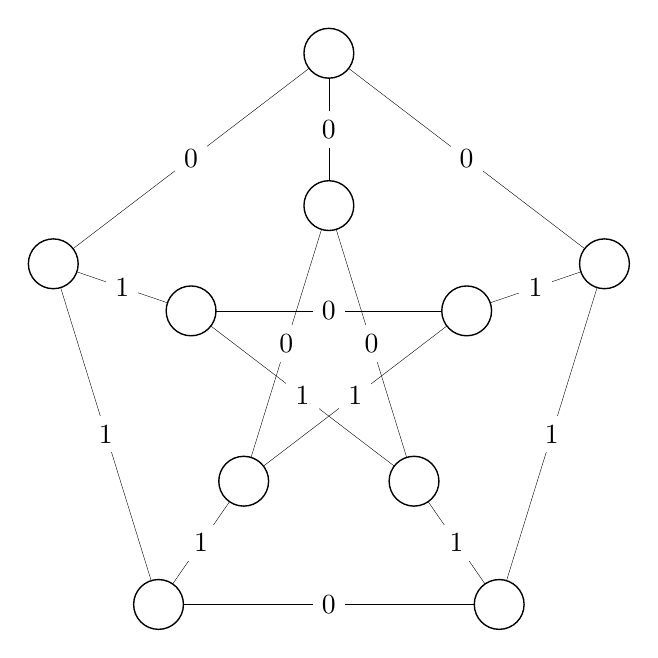
\begin{tikzpicture}
\Vertex[style={minimum size=0.01cm,shape=circle},NoLabel,x=3.5cm,y=7.0cm]{v0}
\Vertex[style={minimum size=0.01cm,shape=circle},NoLabel,x=0.0cm,y=4.3262cm]{v1}
\Vertex[style={minimum size=0.01cm,shape=circle},NoLabel,x=1.3369cm,y=0.0cm]{v2}
\Vertex[style={minimum size=0.01cm,shape=circle},NoLabel,x=5.6631cm,y=0.0cm]{v3}
\Vertex[style={minimum size=0.01cm,shape=circle},NoLabel,x=7.0cm,y=4.3262cm]{v4}
\Vertex[style={minimum size=0.01cm,shape=circle},NoLabel,x=3.5cm,y=5.0652cm]{v5}
\Vertex[style={minimum size=0.01cm,shape=circle},NoLabel,x=1.75cm,y=3.7284cm]{v6}
\Vertex[style={minimum size=0.01cm,shape=circle},NoLabel,x=2.4184cm,y=1.5652cm]{v7}
\Vertex[style={minimum size=0.01cm,shape=circle},NoLabel,x=4.5816cm,y=1.5652cm]{v8}
\Vertex[style={minimum size=0.01cm,shape=circle},NoLabel,x=5.25cm,y=3.7284cm]{v9}
%
\Edge[lw=0.005cm,labelstyle={pos=0.5,},label=\hbox{$0$},](v0)(v1)
\Edge[lw=0.005cm,labelstyle={pos=0.5,},label=\hbox{$0$},](v0)(v4)
\Edge[lw=0.005cm,labelstyle={pos=0.5,},label=\hbox{$0$},](v0)(v5)
\Edge[lw=0.005cm,labelstyle={pos=0.5,},label=\hbox{$1$},](v1)(v2)
\Edge[lw=0.005cm,labelstyle={pos=0.5,},label=\hbox{$1$},](v1)(v6)
\Edge[lw=0.005cm,labelstyle={pos=0.5,},label=\hbox{$0$},](v2)(v3)
\Edge[lw=0.005cm,labelstyle={pos=0.5,},label=\hbox{$1$},](v2)(v7)
\Edge[lw=0.005cm,labelstyle={pos=0.5,},label=\hbox{$1$},](v3)(v4)
\Edge[lw=0.005cm,labelstyle={pos=0.5,},label=\hbox{$1$},](v3)(v8)
\Edge[lw=0.005cm,labelstyle={pos=0.5,},label=\hbox{$1$},](v4)(v9)
\Edge[lw=0.005cm,labelstyle={pos=0.5,},label=\hbox{$0$},](v5)(v7)
\Edge[lw=0.005cm,labelstyle={pos=0.5,},label=\hbox{$0$},](v5)(v8)
\Edge[lw=0.005cm,labelstyle={pos=0.5,},label=\hbox{$1$},](v6)(v8)
\Edge[lw=0.005cm,labelstyle={pos=0.5,},label=\hbox{$0$},](v6)(v9)
\Edge[lw=0.005cm,labelstyle={pos=0.5,},label=\hbox{$1$},](v7)(v9)
%
\end{tikzpicture} 

}
\end{center}
\end{frame}

\begin{frame}
  \frametitle{Coding.} 
  
    Another Example, the repttion code can be thought as the tanner graph defind by the parity code on the cyle graph.
    \begin{center}
      \scalebox{0.7}{
      \begin{tikzpicture}[scale=1]
      \draw
        (8.0, 0.0) node[shape=circle,draw=black] (0){}
        (7.825, 0.624) node[shape=circle,draw=black] (1){}
        (7.308, 1.22) node[shape=circle,draw=black] (2){}
        (6.472, 1.763) node[shape=circle,draw=black] (3){}
        (5.353, 2.229) node[shape=circle,draw=black] (4){}
        (4.0, 2.598) node[shape=circle,draw=black] (5){}
        (2.472, 2.853) node[shape=circle,draw=black] (6){}
        (0.836, 2.984) node[shape=circle,draw=black] (7){}
        (-0.836, 2.984) node[shape=circle,draw=black] (8){}
        (-2.472, 2.853) node[shape=circle,draw=black] (9){}
        (-4.0, 2.598) node[shape=circle,draw=black] (10){}
        (-5.353, 2.229) node[shape=circle,draw=black] (11){}
        (-6.472, 1.763) node[shape=circle,draw=black] (12){}
        (-7.308, 1.22) node[shape=circle,draw=black] (13){}
        (-7.825, 0.624) node[shape=circle,draw=black] (14){}
        (-8.0, 0.0) node[shape=circle,draw=black] (15){}
        (-7.825, -0.624) node[shape=circle,draw=black] (16){}
        (-7.308, -1.22) node[shape=circle,draw=black] (17){}
        (-6.472, -1.763) node[shape=circle,draw=black] (18){}
        (-5.353, -2.229) node[shape=circle,draw=black] (19){}
        (-4.0, -2.598) node[shape=circle,draw=black] (20){}
        (-2.472, -2.853) node[shape=circle,draw=black] (21){}
        (-0.836, -2.984) node[shape=circle,draw=black] (22){}
        (0.836, -2.984) node[shape=circle,draw=black] (23){}
        (2.472, -2.853) node[shape=circle,draw=black] (24){}
        (4.0, -2.598) node[shape=circle,draw=black] (25){}
        (5.353, -2.229) node[shape=circle,draw=black] (26){}
        (6.472, -1.763) node[shape=circle,draw=black] (27){}
        (7.308, -1.22) node[shape=circle,draw=black] (28){}
        (7.825, -0.624) node[shape=circle,draw=black] (29){};
      \begin{scope}[-,draw opacity=0.5]
        \draw (0) to node[] {$1$} (1);
        \draw (0) to node[] {$1$} (29);
        \draw (1) to node[] {$1$} (2);
        \draw (2) to node[] {$1$} (3);
        \draw (3) to node[] {$1$} (4);
        \draw (4) to node[] {$1$} (5);
        \draw (5) to node[] {$1$} (6);
        \draw (6) to node[] {$1$} (7);
        \draw (7) to node[] {$1$} (8);
        \draw (8) to node[] {$1$} (9);
        \draw (9) to node[] {$1$} (10);
        \draw (10) to node[] {$1$} (11);
        \draw (11) to node[] {$1$} (12);
        \draw (12) to node[] {$1$} (13);
        \draw (13) to node[] {$1$} (14);
        \draw (14) to node[] {$1$} (15);
        \draw (15) to node[] {$1$} (16);
        \draw (16) to node[] {$1$} (17);
        \draw (17) to node[] {$1$} (18);
        \draw (18) to node[] {$1$} (19);
        \draw (19) to node[] {$1$} (20);
        \draw (20) to node[] {$1$} (21);
        \draw (21) to node[] {$1$} (22);
        \draw (22) to node[] {$1$} (23);
        \draw (23) to node[] {$1$} (24);
        \draw (24) to node[] {$1$} (25);
        \draw (25) to node[] {$1$} (26);
        \draw (26) to node[] {$1$} (27);
        \draw (27) to node[] {$1$} (28);
        \draw (28) to node[] {$1$} (29);
      \end{scope}
    \end{tikzpicture}
 
  }
  \end{center}
  \end{frame}


  \begin{frame}
    \frametitle{ Quantum Error Correction Codes. }
    Back to the quantum noise. 
%    \begin{equation*}
%      \begin{split}
%        
%      \end{split}
%    \end{equation*}<++>
%

  \end{frame} 

\begin{frame}
  \frametitle{ Quantum Noise. }
  \begin{center}
  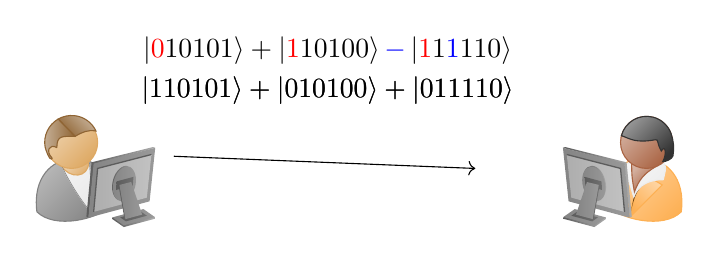
\begin{tikzpicture}
    \node[name=b, bob,monitor,minimum size=1cm,xshift=-7.2cm]{};
    \node[name= a, alice,monitor, mirrored,minimum size=1cm]{};
    \node (C) at (-2,0) {};
    \draw[ -> ] (b.mouth) + (1,0) to (C)  ; 
    \alt<3->{ 
      \node(D) at (-4,1.5) { $\ket{\textcolor{red}{0}10101} + \ket{\textcolor{red}{1}10100} \textcolor{blue}{-} \ket{\textcolor{red}{1}1\textcolor{blue}{1}110}$} ;
  \node(E) at (-4,1) { $\ket{110101} + \ket{010100} + \ket{011110}$} ;
  }{
      \node(D) at (-4,1) { $\ket{110101} + \ket{010100} + \ket{011110}$} ;
    }
    %\uncover<2->{\node (D) at (-4,1) { $110101$ } ;  
  \end{tikzpicture}
\end{center}
\end{frame}


\begin{frame}
  \frametitle{ Quantum Error Correction Codes. }

\begin{definition}[CSS Code]
  Let $C_{X}, C_{Z}$ classical linear codes such that $C_{Z}^{\perp} \subset C_{X}$ define the $Q\left( C_{X},C_{Z} \right)$ to be all the codewords with following structure:
  \begin{equation*}
    \begin{split}
    \ket { \mathbf{ x } } := \ket { x + C_{Z}^{\perp} } = \frac{1}{\sqrt{C_{Z}^{\perp}}} \sum_{z \in C_{Z}^{\perp}}{ \ket{ x + z }} 
    \end{split}
  \end{equation*}
\end{definition}
\end{frame} 

\begin{frame}
  \frametitle{ Quantum Error Correction Codes. }
  \begin{center}
    \begin{figure}[H]
  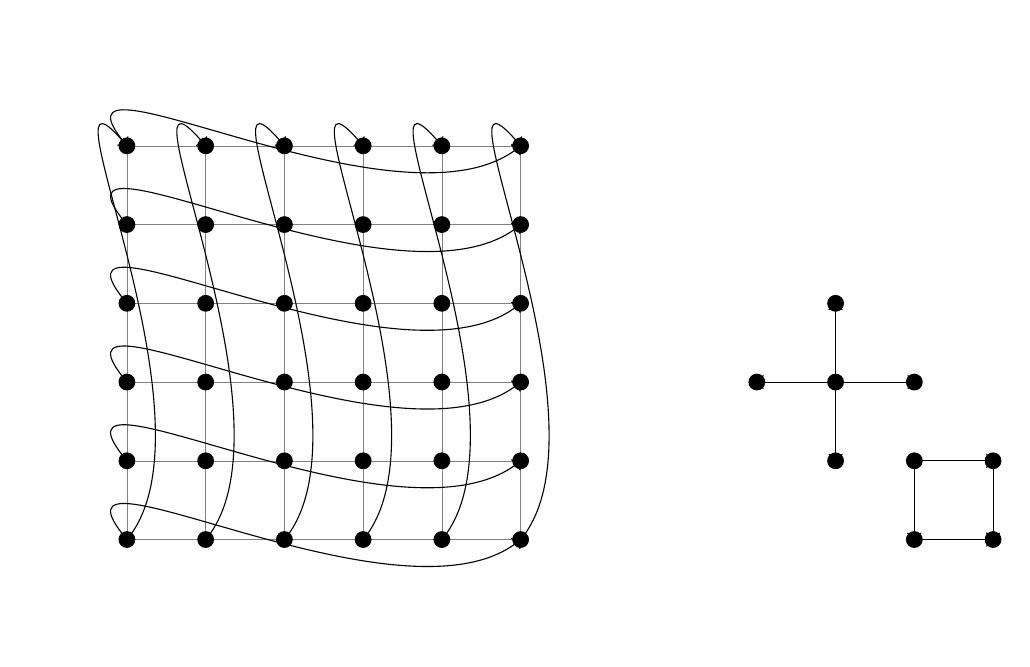
\begin{tikzpicture}
  \draw[step=1cm,gray,very thin] (0,0) grid (5,5);
  \foreach \x in {0,1,2,3,4,5}
  \foreach \y in {0,1,2,3,4,5}
  {
  \node[draw,circle,inner sep=2pt,fill] at (\x,\y) {};
}
\draw[ -> ]  (0,0) to [out=50, in=130] (0,5);
\draw[ -> ]  (1,0) to [out=50, in=130] (1,5);
\draw[ -> ]  (2,0) to [out=50, in=130] (2,5);
\draw[ -> ]  (3,0) to [out=50, in=130] (3,5);
\draw[ -> ]  (4,0) to [out=50, in=130] (4,5);
\draw[ -> ]  (5,0) to [out=50, in=130] (5,5);
\draw[ -> ]  (0,5) to [out=130, in=220] (5,5);
\draw[ -> ]  (0,4) to [out=130, in=220] (5,4);
\draw[ -> ]  (0,3) to [out=130, in=220] (5,3);
\draw[ -> ]  (0,2) to [out=130, in=220] (5,2);
\draw[ -> ]  (0,1) to [out=130, in=220] (5,1);
\draw[ -> ]  (0,0) to [out=130, in=220] (5,0);

\node[draw,circle,inner sep=2pt,fill] at (9,2) {};
\node[draw,circle,inner sep=2pt,fill] at (10,2) {};
\node[draw,circle,inner sep=2pt,fill] at (8,2) {};
\node[draw,circle,inner sep=2pt,fill] at (9,1) {};
\node[draw,circle,inner sep=2pt,fill] at (9,3) {};
\draw[ -> ]  (9,2) to (10,2);
\draw[ -> ]  (9,2) to (8,2);
\draw[ -> ]  (9,2) to (9,1);
\draw[ -> ]  (9,2) to (9,3);
%\draw[ -> ]  (9,2) to (5,0);

\node[draw,circle,inner sep=2pt,fill] at (10,1) {};
\node[draw,circle,inner sep=2pt,fill] at (11,1) {};
\node[draw,circle,inner sep=2pt,fill] at (10,0) {};
\node[draw,circle,inner sep=2pt,fill] at (11,0) {};
\draw[ -> ]  (10,1) to (11,1);
\draw[ -> ]  (10,1) to (10,0);
\draw[ -> ]  (10,0) to (11,0);
\draw[ -> ]  (11,1) to (11,0);
\end{tikzpicture}
\caption{On the left is the Toric Graph. On the right are cross and face checks.}
\label{fig:Toric}
\end{figure}
\end{center}

\end{frame} 

\begin{frame}
  \frametitle{ Quantum Error Correction Codes. }
\begin{definition}[$w$-Robustness] 
  \label{def:wrobust}
  Let $C_{A}$ and $C_{B}$ be codes of length $\Delta$ with minimum distance $\delta_{0}\Delta$. $C = \duC $ will be said to be $w$-robust if for any codeword $c \in C$ of weight less than $w$, it follows that $c$ can be decomposed into a sum of $c = t + s$ such that $t \in C_A \otimes \mathbb{F}^{B}$ and $s \in \mathbb{F}^A \otimes C_B$, where $s$ and $t$ are each supported on at most $\frac{w}{\delta_0\Delta}$ rows and columns. For convenience, we will denote by $B'$ ($A'$) the rows (columns) supporting $t$ ($s$) and use the notation $t \in C_A \otimes \mathbb{F}^{B'}$.
\end{definition}
\end{frame} 

\begin{frame}
  \frametitle{ Quantum Error Correction Codes. }
  \begin{center}
  \scalebox{0.65}{
  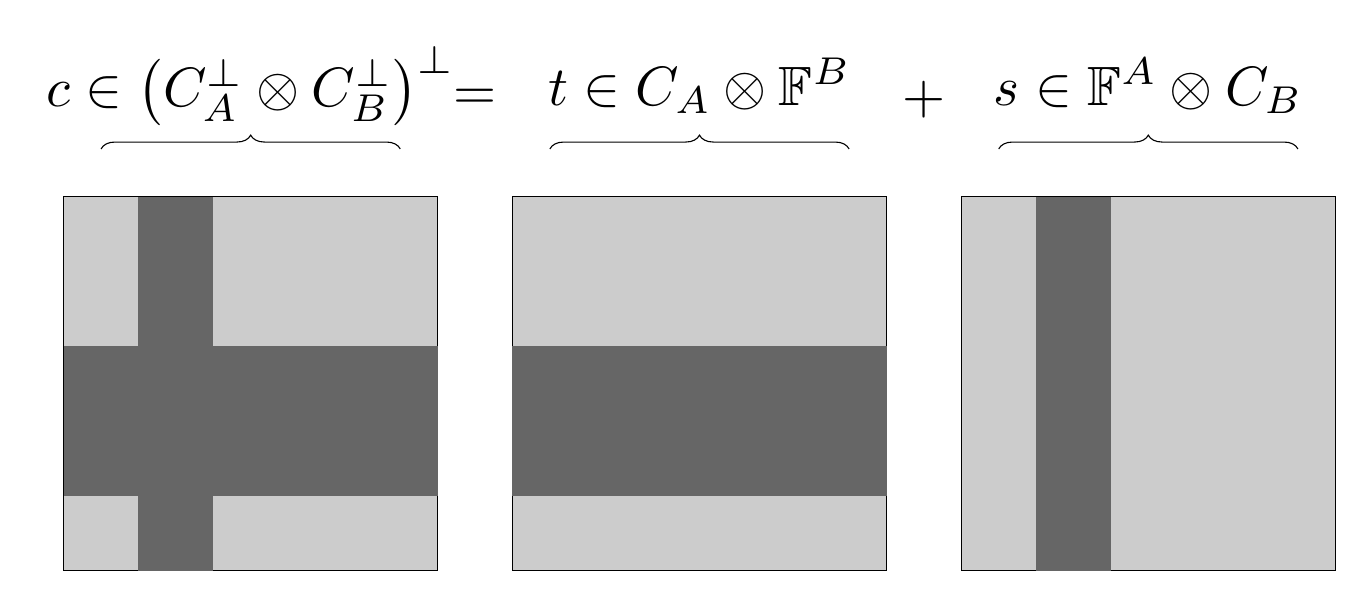
\begin{tikzpicture}[scale=0.95]

\draw (5.5,6.3) node[scale=2]  { $=$ };
\draw (11.5,6.3) node[scale=2]  { $+$ };

\draw [decorate,decoration={brace,amplitude=5pt,raise=4ex}] 
(0.5,5) -- (4.5,5) node[scale=2,midway,yshift=2em]{$c \in \left(C_{A}^{\perp}\otimes C_{B}^{\perp}\right)^{\perp} $};
    \filldraw [fill=white!80!black](0,0) rectangle (5,5);
   \fill [fill=gray!80!black] (1,0) rectangle (2,5);
    \fill [fill=gray!80!black] (0,1) rectangle (5,3);
\filldraw [fill=white!80!black](6,0) rectangle (11,5);
\draw [decorate,decoration={brace,amplitude=5pt,raise=4ex}] 
(6.5,5) -- (10.5,5) node[scale=2,midway,yshift=2em]{$t \in C_{A}\otimes \mathbb{F}^{B}$};
   \fill [fill=gray!80!black,draw opacity=0.5] (6,1) rectangle (11,3);
\filldraw [fill=white!80!black](12,0) rectangle (17,5);
\draw [decorate,decoration={brace,amplitude=5pt,raise=4ex}] 
(12.5,5) -- (16.5,5) node[scale=2,midway,yshift=2em]{$s \in \mathbb{F}^{A}\otimes C_{B}$};
 \fill [fill=gray!80!black,draw opacity=0.5] (13,0) rectangle (14,5);
        \end{tikzpicture}
      }
    \end{center}
\end{frame} 

\begin{frame}
  \frametitle{ Quantum Error Correction Codes. }
  \begin{center}
  \scalebox{0.55}{
      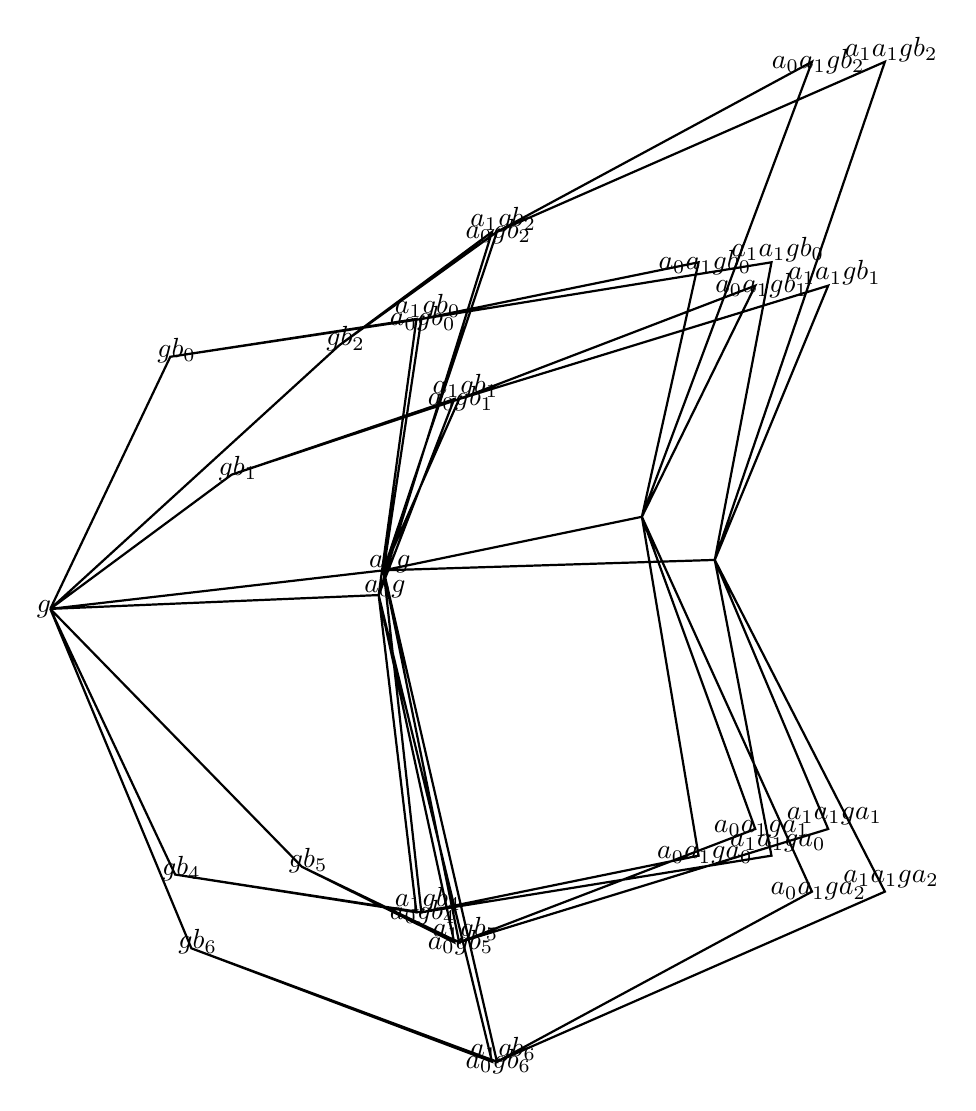
\begin{tikzpicture}[scale=0.8]
            \draw[thick](0,0)(0, 0) -- (1.9049911888377424,4.002079117547451) -- (5.81285084955138,4.602079117547451) -- (5.212850849551381,0.2192498173032679) -- (0, 0)
(0, 0) -- (2.879157898699928,2.130954290533681) -- (6.412850849551381,3.330954290533681) -- (5.212850849551381,0.2192498173032679) -- (0, 0)
(0, 0) -- (4.588270563356833,4.1850314105127575) -- (7.012850849551381,5.985031410512757) -- (5.212850849551381,0.2192498173032679) -- (0, 0)
(0, 0) -- (1.9049911888377424,4.002079117547451) -- (5.890590913653101,4.602079117547451) -- (5.2905909136531015,0.6119546131629411) -- (0, 0)
(0, 0) -- (2.879157898699928,2.130954290533681) -- (6.490590913653102,3.330954290533681) -- (5.2905909136531015,0.6119546131629411) -- (0, 0)
(0, 0) -- (4.588270563356833,4.1850314105127575) -- (7.090590913653101,5.985031410512757) -- (5.2905909136531015,0.6119546131629411) -- (0, 0)
(0, 0) -- (1.9818949186177792,-4.217396385887875) -- (5.81285084955138,-4.817396385887875) -- (5.212850849551381,0.2192498173032679) -- (0, 0)
(0, 0) -- (3.9944175473955323,-4.094159016671296) -- (6.412850849551381,-5.294159016671296) -- (5.212850849551381,0.2192498173032679) -- (0, 0)
(0, 0) -- (2.2401823432002748,-5.388664191428558) -- (7.012850849551381,-7.188664191428558) -- (5.212850849551381,0.2192498173032679) -- (0, 0)
(0, 0) -- (1.9818949186177792,-4.217396385887875) -- (5.890590913653101,-4.817396385887875) -- (5.2905909136531015,0.6119546131629411) -- (0, 0)
(0, 0) -- (3.9944175473955323,-4.094159016671296) -- (6.490590913653102,-5.294159016671296) -- (5.2905909136531015,0.6119546131629411) -- (0, 0)
(0, 0) -- (2.2401823432002748,-5.388664191428558) -- (7.090590913653101,-7.188664191428558) -- (5.2905909136531015,0.6119546131629411) -- (0, 0)
(5.2905909136531015, 0.6119546131629411) -- (5.890590913653101,4.602079117547451) -- (10.291575076901802,5.502079117547451) -- (9.391575076901802,1.4619219538089987) -- (5.2905909136531015, 0.6119546131629411)
(5.2905909136531015, 0.6119546131629411) -- (6.490590913653102,3.330954290533681) -- (11.191575076901803,5.130954290533681) -- (9.391575076901802,1.4619219538089987) -- (5.2905909136531015, 0.6119546131629411)
(5.2905909136531015, 0.6119546131629411) -- (7.090590913653101,5.985031410512757) -- (12.091575076901801,8.685031410512757) -- (9.391575076901802,1.4619219538089987) -- (5.2905909136531015, 0.6119546131629411)
(5.2905909136531015, 0.6119546131629411) -- (5.890590913653101,4.602079117547451) -- (11.4486392380322,5.502079117547451) -- (10.5486392380322,0.7771825477033486) -- (5.2905909136531015, 0.6119546131629411)
(5.2905909136531015, 0.6119546131629411) -- (6.490590913653102,3.330954290533681) -- (12.3486392380322,5.130954290533681) -- (10.5486392380322,0.7771825477033486) -- (5.2905909136531015, 0.6119546131629411)
(5.2905909136531015, 0.6119546131629411) -- (7.090590913653101,5.985031410512757) -- (13.248639238032201,8.685031410512757) -- (10.5486392380322,0.7771825477033486) -- (5.2905909136531015, 0.6119546131629411)
(5.2905909136531015, 0.6119546131629411) -- (5.890590913653101,-4.817396385887875) -- (10.291575076901802,-3.917396385887875) -- (9.391575076901802,1.4619219538089987) -- (5.2905909136531015, 0.6119546131629411)
(5.2905909136531015, 0.6119546131629411) -- (6.490590913653102,-5.294159016671296) -- (11.191575076901803,-3.494159016671296) -- (9.391575076901802,1.4619219538089987) -- (5.2905909136531015, 0.6119546131629411)
(5.2905909136531015, 0.6119546131629411) -- (7.090590913653101,-7.188664191428558) -- (12.091575076901801,-4.488664191428557) -- (9.391575076901802,1.4619219538089987) -- (5.2905909136531015, 0.6119546131629411)
(5.2905909136531015, 0.6119546131629411) -- (5.890590913653101,-4.817396385887875) -- (11.4486392380322,-3.917396385887875) -- (10.5486392380322,0.7771825477033486) -- (5.2905909136531015, 0.6119546131629411)
(5.2905909136531015, 0.6119546131629411) -- (6.490590913653102,-5.294159016671296) -- (12.3486392380322,-3.494159016671296) -- (10.5486392380322,0.7771825477033486) -- (5.2905909136531015, 0.6119546131629411)
(5.2905909136531015, 0.6119546131629411) -- (7.090590913653101,-7.188664191428558) -- (13.248639238032201,-4.488664191428557) -- (10.5486392380322,0.7771825477033486) -- (5.2905909136531015, 0.6119546131629411)
;
\node at (5.91285084955138,4.602079117547451) {$ a_{ 0  } gb_{ 0 } $};
\node at (6.512850849551381,3.330954290533681) {$ a_{ 0  } gb_{ 1 } $};
\node at (7.11285084955138,5.985031410512757) {$ a_{ 0  } gb_{ 2 } $};
\node at (5.990590913653101,4.802079117547451) {$ a_{ 1  } gb_{ 0 } $};
\node at (6.590590913653101,3.530954290533681) {$ a_{ 1  } gb_{ 1 } $};
\node at (7.190590913653101,6.1850314105127575) {$ a_{ 1  } gb_{ 2 } $};
\node at (5.91285084955138,-4.817396385887875) {$ a_{ 0  } gb_{ 4 } $};
\node at (6.512850849551381,-5.294159016671296) {$ a_{ 0  } gb_{ 5 } $};
\node at (7.11285084955138,-7.188664191428558) {$ a_{ 0  } gb_{ 6 } $};
\node at (5.990590913653101,-4.617396385887875) {$ a_{ 1  } gb_{ 4 } $};
\node at (6.590590913653101,-5.094159016671296) {$ a_{ 1  } gb_{ 5 } $};
\node at (7.190590913653101,-6.988664191428557) {$ a_{ 1  } gb_{ 6 } $};
\node at (10.391575076901802,5.502079117547451) {$ a_{ 0  } a_{ 1 }gb_{ 0 } $};
\node at (11.291575076901802,5.130954290533681) {$ a_{ 0  } a_{ 1 }gb_{ 1 } $};
\node at (12.1915750769018,8.685031410512757) {$ a_{ 0  } a_{ 1 }gb_{ 2 } $};
\node at (11.5486392380322,5.702079117547451) {$ a_{ 1  } a_{ 1 }gb_{ 0 } $};
\node at (12.4486392380322,5.330954290533681) {$ a_{ 1  } a_{ 1 }gb_{ 1 } $};
\node at (13.3486392380322,8.885031410512756) {$ a_{ 1  } a_{ 1 }gb_{ 2 } $};
\node at (10.391575076901802,-3.917396385887875) {$ a_{ 0  } a_{ 1 }ga_{ 0 } $};
\node at (11.291575076901802,-3.494159016671296) {$ a_{ 0  } a_{ 1 }ga_{ 1 } $};
\node at (12.1915750769018,-4.488664191428557) {$ a_{ 0  } a_{ 1 }ga_{ 2 } $};
\node at (11.5486392380322,-3.717396385887875) {$ a_{ 1  } a_{ 1 }ga_{ 0 } $};
\node at (12.4486392380322,-3.294159016671296) {$ a_{ 1  } a_{ 1 }ga_{ 1 } $};
\node at (13.3486392380322,-4.288664191428557) {$ a_{ 1  } a_{ 1 }ga_{ 2 } $};
\node at (-0.1,0) {$ g $};
\node at (5.31285084955138,0.3192498173032679) {$ a_{ 0 }g $};
\node at (5.390590913653101,0.7119546131629411) {$ a_{ 1 }g $};
\node at (2.0049911888377423,4.102079117547451) {$ gb_{ 0 } $};
\node at (2.979157898699928,2.230954290533681) {$ gb_{ 1 } $};
\node at (4.6882705633568325,4.285031410512757) {$ gb_{ 2 } $};
\node at (2.0818949186177793,-4.117396385887876) {$ gb_{ 4 } $};
\node at (4.094417547395532,-3.9941590166712957) {$ gb_{ 5 } $};
\node at (2.340182343200275,-5.288664191428558) {$ gb_{ 6 } $};          
\end{tikzpicture}}
\end{center}
\end{frame} 

\begin{frame}
  \frametitle{ Quantum Error Correction Codes. }
\begin{definition}[$p$-Resistance to Puncturing.]
%  \label{def:resistance}
  Let $p,w$ be integers. We will say that the dual tensor code $C_{A} \otimes \mathbb{F} + \mathbb{F} \otimes C_{B}$ is $w$-robust with $p$-resistance to puncturing, if the code obtained by removing (puncturing) a subset of at most $p$ rows and columns is $w$-robust.   
\end{definition}
\end{frame} 

\begin{frame}
  \frametitle{ Quantum Error Correction Codes. }
\begin{definition}[Quantum Tanner Code.]

%  Let $\Gamma$ be a group on $n$ verices. And let $A,B$ be a two generator set of $\Gamma$ such that if $a \in A$ ($B$) then also $a^{-1}\in A$ and that for any $g\in \Gamma,a \in A, b \in B$ it holds that $g \neq agb$ . Define the left right Cayley complex to be the graph $G = \left( \Gamma, E \right) $ obtain by taking the union of the two Cayley graphs generated by $A$ and $B$. So the vertices pair $u,v$ are set on square diaginal only if there are $a\in A$ and $b \in B$ such that $u = avb$. We can assume that $G$ is a bipartite graph (otherise just take $\Gamma^{\prime} = \Gamma \times \mathbb{Z}_{2}$ and define the product to be $a\left( u,\pm \right) = \left( au, \mp \right)$). 
%
%  Now divide the graph into postivie and negative vertices according their coloring $V_{-}$ and $V_{+}$. And define the positive graph to be $G^{+} = \left( V_{+}, E \right)$ and by $G^{-} = \left( V_{-}, E \right)$ the negative graph, when $E$denotes the sqaures, put it defrently their is an edge between $v$ and $u$ in $G^{+}$ if both vertices are positive and they are lay on the ends of square's diongal.
%
%  The quantum tanner code is a CSS code, such $C_{X}$ defined to be the classical tanner code $\mathcal{T}\left(G^{+}, \left(C_{A}^\perp\otimes C_{B}^{\perp}\right)^{\perp} \right)$ and $C_{Z}$ define as $\mathcal{T}\left(G^{-}, \left(C_{A}\otimes C_{B}\right)^{\perp} \right)$. Noice that in contrast to classical tanner code, in the quantum case it will be more convinent to think codewords as assiments set on the squaers and not on the edges.  
%
  Let $\Gamma$ be a group at size $n$. And let $A,B$ be a two generator set of $\Gamma$ such that if $a \in A$ ($B$) then also $a^{-1}\in A$ ($B^{-1}$) and that for any $g\in \Gamma, a \in A, b \in B$ it holds that $g \neq agb$. Define the left-right Cayley complex to be the graph $G = \left( \Gamma, E \right)$ obtained by taking the union of the two Cayley graphs generated by $A$ and $B$. So the vertices pair $u,v$ are set on a square diagonal only if there are $a\in A$ and $b \in B$ such that $u = avb$. We can assume that $G$ is a bipartite graph (otherwise just take $\Gamma^{\prime} = \Gamma \times \mathbb{Z}_{2}$ and define the product to be $a\left( u,\pm \right) = \left( au, \mp \right)$).
\end{definition}
\end{frame}


\begin{frame}
  \frametitle{ Quantum Error Correction Codes. }
\begin{definition}[Quantum Tanner Code.]


Now divide the graph into positive and negative vertices according to their coloring $V_{-}$ and $V_{+}$. And define the positive graph to be $G^{+} = \left( V_{+}, E \right)$ and by $G^{-} = \left( V_{-}, E \right)$ the negative graph, where $E$ denotes the squares, put differently there is an edge between $v$ and $u$ in $G^{+}$ if both vertices are positive and they are laid on the ends of a square's diagonal.


The quantum Tanner code is a CSS code, such that $C_{X}$ is defined to be the classical Tanner code $\mathcal{T}\left(G^{+}, \left(C_{A}^\perp\otimes C_{B}^{\perp}\right)^{\perp} \right)$ and $C_{Z}$ is defined as $\mathcal{T}\left(G^{-}, \left(C_{A}\otimes C_{B}\right)^{\perp} \right)$. Note that in contrast to the classical Tanner code, in the quantum case it will be more convenient to think of codewords as assignments set on the squares and not on the edges.
\end{definition}

\end{frame} 

\begin{frame}
  \frametitle{ Quantum Error Correction Codes. }
\end{frame} 



\end{document}
